\documentclass{ddis-thesis}
\usepackage{amsmath, amsthm, amssymb}
\usepackage[utf8]{inputenc}
\usepackage{program}
\usepackage{mathrsfs}
\usepackage{amsfonts}

\usepackage{fancyvrb}
\DefineVerbatimEnvironment{code}{Verbatim}{fontsize=\small}
\DefineVerbatimEnvironment{example}{Verbatim}{fontsize=\small}


\usepackage{fancyhdr}% fancyhdr related command; details in its documentation
\pagestyle{fancy}
\fancyhead{}
\fancyhead[LE,RO]{\thepage}
\fancyhead[RE]{\leftmark}
\fancyhead[LO]{\rightmark}


\usepackage{graphicx}
\author{name}
\title{Thesis title}
\begin{document}

% *************** Front matter ***************

\frontmatter
\begin{titlepage}

\setlength{\textwidth}{16cm}
\setlength{\oddsidemargin}{0cm}
\setlength{\evensidemargin}{0cm}
\setlength{\topmargin}{8mm}
\setlength{\headheight}{0cm}
\setlength{\headsep}{0cm}
\setlength{\topskip}{0cm}
\enlargethispage{5cm}

\noindent
\setlength{\unitlength}{1mm}

\begin{picture}(160,226)
\centering

\put(0,203){\line(1,0){160}} % lower line
\put(109,39){\line(1,0){50}}
\put(109,161){\line(1,0){50}}
\put(109,170){\line(1,0){50}}
\put(107,1){\line(0,1){200}}

\put(0,140){\parbox[b][6em]{100mm}{
    \begin{center}
    \textbf{\Huge{\sffamily{Analysis of Weather Data using Graph-based and Neural Network Methods}}}
    \end{center}}}

\put(109,92){\parbox[b]{50mm}{
    \textbf{{\sffamily{{\Large Roland Schl\"afli}}}}\\
    {\sffamily{of Bern BE, Switzerland\\\\
    Student-ID: 12-932-398\\
    rolandschlaefli@gmail.com
    }}
}}

\put(109,161){\makebox(50,9){{\sffamily{BSc Thesis \hfill January 31, 2018}}}}

\put(0,215){\makebox(80,11)[l]{
\includegraphics[height=2.8cm]
{./00_title/figures/uzh_logo_e_pos}}}


\put(109,32){\parbox[b]{50mm}{\flushleft
    {\sffamily{Advisor:}} {\textbf{\sffamily{Bibek Paudel}} }
    }
}

\put(109,10){\parbox[b]{50mm}{\flushleft
        {\sffamily{
        Prof. Abraham Bernstein, PhD\\
        Institut f\"ur Informatik\\
        Universit\"at Z\"urich\\
        http://www.ifi.uzh.ch/ddis}
        }
}}

\end{picture}
\end{titlepage}



\begin{acknowledgements}
First and foremost, I would like to thank Prof. Bernstein for the opportunity to work on such an interesting problem at his research group.

I am also very grateful for the tremendous support provided by my advisor Bibek Paudel, who was always ready to provide constructive feedback and new ideas. His support made the overall creation of this work a thoroughly enjoyable and interesting process.

I would further like to thank Veronika Stolbova for her willingness to consult with us on our early approaches and results, which has helped us identify some early flaws in our implementation. My thanks also go out to Anja Zgraggen and Pascal Zehnder, who have helped improve the formal and content-related correctness of this work.
\end{acknowledgements}

\begin{zusammenfassung}
Der Indische Sommermonsun ist von grosser Bedeutung für über eine Milliarde Menschen. Die Wichtigkeit einer präzisen statistischen Auswertung des Monsunverhaltens wird dadurch deutlich. In dieser Arbeit analysieren wir die geographische Verteilung von extremem Monsunregenfall und entwickeln eine neue Methode zur Vorhersage des Monsunbeginns. Wir berechnen Netzwerke aus korrelierten Orten auf dem Indischen Subkontinent und analysieren diese mit verbreiteten Indikatoren der Netzwerkzentralität. Dadurch zeigt sich eine relative Wichtigkeit von Regionen wie dem Indischen Ozean, dem Tibetischen Plateau und Nordpakistan. Basierend auf aktuellen Methoden im Bereich der Neuronalen Netzwerke entwickeln wir ausserdem ein neues Modell zur Vorhersage des Monsunbeginns basierend auf räumlich-zeitlichen Wetterdaten. Mit darauf aufbauenden Experimenten zeigen wir, dass unser Modell den Monsunanfang mehrere Tage im Voraus genauer als bestehende Methoden vorhersagen kann.
\end{zusammenfassung}

\begin{abstract}
Each year, the Indian Summer Monsoon affects more than one billion people, making clear the importance of accurate statistical analysis of its behavior. In this work, we analyze the spatial distribution of extreme monsoon rainfall and propose a new way of predicting monsoon onset dates. We build networks of correlated locations on the Indian subcontinent, analyzing them with established centrality measures. These centrality measures reveal the relative importance of locations like the Indian Ocean, the Tibetan Plateau, and Northern Pakistan. We additionally adopt recent advances in machine learning and neural networks to predict monsoon onset dates based on spatiotemporal meteorological datasets. With experiments on these datasets, we show that our model is able to predict onset dates more accurately than existing methods several days in advance.
\end{abstract}


\tableofcontents

% *************** Main matter ***************
\mainmatter

\chapter{Introduction}
\label{c:introduction}

The Indian Summer Monsoon (further also referred to as ISM) is one of the most significant meteorological events on our planet. It shapes the lives of the more than one billion people living in and around India. Many parts of India receive up to 80\% of rainfall during the monsoon season, and significant parts of the population obtain their drinking water from monsoon rainfalls \citep{Stolbova.2015}. Farmers further depend on the arrival of these rainfalls to be able to water their crops and feed their livestock. The monsoon is of similarly high impact for the Indian economy at large, as the country is still dependent on its agricultural sector, which makes up almost one-fifth of India's GDP \citep{CentralIntelligenceAgency.05.01.2018}.

In itself, the ISM is a highly complex climatological phenomenon. It displays considerable variability in both timing and strength and is influenced by many factors on regional and global scales. Due to its obvious importance, the behavior of the ISM has been a focus of climate researchers for many decades, bringing to light many theories and hypotheses. However, even today, some of its characteristics and global teleconnections remain unexplained.

[TODO: extend "motivation"]

Because of the complex behavior of the ISM, we dedicate \cref{c:ism_overview} of this work to a short summarization of research about the inner workings of the ISM. We explain the major factors that are known to influence monsoon as well as theories for those that are still unknown. We also try to further motivate the significance and social impact of the monsoon for the people in India and its surrounding countries.

\begin{figure}[h]
  \centering
  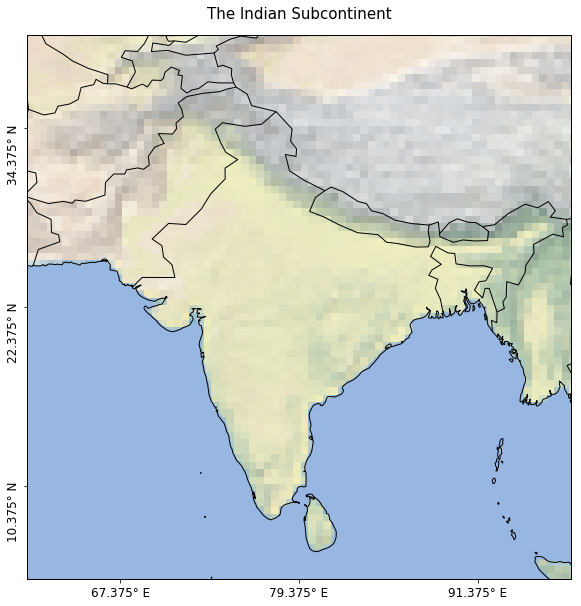
\includegraphics[width=0.5\linewidth]{./99_appendix/img/area_overview}
  \caption{The Indian subcontinent as extracted from TRMM.}
  \label{fig:trmm_area}
\end{figure}

The remainder of this work is then structured into two major parts that are both firmly connected to the behavior of the ISM. The first part (\cref{c:event_sync}) is dedicated to the analysis of extreme precipitation\footnote{Rainfall} events before, during and after the monsoon season. Such events are regularly seen all over India and represent one of the most significant challenges the local population faces from the ISM. Extreme rainfall can cause enormous damage by flooding cities or destruction of essential infrastructure. As such, there is a clear need to analyze and predict the spatial and temporal distribution of these extreme rainfall events.

Strongly basing our first part on the work of \citet{Stolbova.2015}, we extract extreme rainfall events from the TRMM precipitation dataset.

[TODO: short TRMM summary]

We then calculate the synchronicity of different pairs of locations\footnote{Simplified example: two locations are synchronous if an extreme event in one location tends to be followed by an extreme event in the other location.} and build a graph (a ``climate network'') connecting the most significantly synchronous locations.

Analysis of the resulting graph using graph centrality measures\footnote{Degree, Betweenness and PageRank} finally shows us the locations that are the most central and important in the graph. This knowledge could potentially help in the analysis or even prediction of monsoon behavior. For example, extreme rainfall in a location that is very central might be a reason to implement additional safety measures in connected locations.

The second major part of this work (\cref{c:part2}) deals with another critical issue regarding the Indian Summer Monsoon: the prediction of the onset date of monsoon. The onset date for a location in India depicts the point at which the monsoon reaches said location with strength and durability above a predefined threshold. We try to predict such an onset date for the Kerala region, which is generally one of the first locations reached by the ISM and as such marks the beginning of monsoon for the whole Indian subcontinent.

[TODO: short ERA-Interim summary]

For our onset prediction task, we build several neural network architectures using the Python Keras 2.0 and Tensorflow 1.4 libraries and describe the intuition of each. Experiments with each model allow us to evaluate and shortly summarize our most important findings. We iteratively improve upon the findings of each model, building models with vastly different architectures as well as for a number of datasets, features and combinations thereof (TRMM, ERA-Interim, different sets of onset dates). An overview and comparison of the learning capabilities of all models then serves as a conclusion to the second part.

Finally concluding our work in \cref{c:conclusion}, we summarize our overall findings and try to interpret the results of \cref{c:event_sync} and \cref{c:part2}. We additionally provide ideas for the improvement of our work and possible future research based on the topics of extreme event synchronization and monsoon onset prediction using neural networks.

\chapter{The First Chapter Title}
\label{c:chapter1} Lorem ipsum dolor sit amet, consectetuer adipiscing elit.
Nullam a tellus. Aliquam commodo dui non ipsum. Duis mollis nisi id turpis.
Donec quis ipsum. Curabitur sed nibh. Morbi suscipit justo quis orci. Ut massa
tortor, ultricies vitae, lacinia eu, facilisis eu, nisl. Nulla mattis urna sed
metus imperdiet ornare. Praesent sodales. Etiam laoreet. Mauris quam magna,
sagittis et, pharetra eget, congue vitae, arcu. Fusce sollicitudin justo.
Suspendisse lectus. Sed lobortis dolor quis lectus scelerisque ornare. Integer
purus. Phasellus vel elit at nibh sagittis lobortis. Aliquam iaculis malesuada
eros. Mauris metus.

Curabitur malesuada, pede aliquam ultrices eleifend, arcu augue cursus pede,
vel gravida velit mauris nec sem. Etiam commodo metus vel velit. Nam aliquet
tortor ut elit. Praesent sodales, lectus sit amet interdum vulputate, augue
libero pretium ipsum, id congue tellus nisi posuere sem. Cras non tellus at
magna porttitor hendrerit. Donec vehicula fermentum enim. Phasellus vel tortor
in tellus varius condimentum. Nullam rhoncus. Morbi molestie laoreet turpis.
Nulla ut erat. Morbi pharetra. Phasellus cursus rutrum nisl. In est. Nunc eu
elit et purus bibendum interdum. Integer elit. Aliquam nec felis.

\section{First Section}
\label{st:section1} Integer congue luctus justo. Curabitur libero dui,
mollis nec, tempor vel, faucibus sit amet, massa. Fusce arcu elit, blandit sed,
placerat venenatis, hendrerit ac, elit. Suspendisse potenti. Etiam non felis
nec enim venenatis adipiscing. Nulla ante. Fusce dolor. Vivamus accumsan
pellentesque eros. Maecenas pede nisl, ullamcorper vitae, venenatis sit amet,
nonummy quis, enim. Ut in risus. Aenean nisi nisi, ullamcorper ut, posuere sit
amet, posuere ut, turpis. Duis at est. Integer aliquam. Sed eget justo at sem
hendrerit fermentum. Sed felis. Vestibulum tellus diam, interdum vel, vehicula
sit amet, egestas et, lacus. Curabitur cursus felis vel sapien. In rhoncus nisi
at orci. In lobortis varius nisi. Etiam ullamcorper libero sit amet felis.

Duis fermentum nonummy enim. In faucibus nunc. Quisque quis sem vitae ante
condimentum imperdiet. Donec malesuada, eros non ornare sagittis, turpis pede
hendrerit turpis, eu vestibulum mi neque ut justo. Nulla in enim eu enim auctor
bibendum. Suspendisse in nunc. Ut adipiscing elit eu. (Figure\ref{f:fig1}).

\subsection{First Subsection}
\label{sst:subsection1} In tellus mauris, nonummy eget, vestibulum in,
interdum at, nulla. Vestibulum eu justo. Vivamus lobortis pellentesque arcu.
Aliquam enim risus, pulvinar quis, pulvinar tempor, pharetra vitae, dolor.
Aliquam ac sapien. Aenean augue eros, malesuada nec, tincidunt eget, aliquet
bibendum, odio. Maecenas eu est eu nisi pulvinar bibendum. Lorem ipsum dolor
sit amet, consectetuer adipiscing elit. Pellentesque eleifend varius enim. Ut
pharetra diam ac nulla. Aliquam a turpis ac mi semper porttitor. Vivamus
sodales molestie nibh. Vivamus in sapien sit amet mauris sagittis lobortis.
Aenean pretium. Suspendisse eu leo at quam vehicula aliquam. Nunc a ipsum. Sed
placerat fringilla nibh. Aliquam sagittis. Integer a augue vitae libero
elementum pretium. Proin metus (see Figure \ref{f:fig2}).

Figure environment.
\begin{figure}[!ht]
\centering

\includegraphics[width=\linewidth]{./section-chapter1/figures/uzh_logo_e_pos.pdf}
\caption[Graphics description ABC]
{Graphics description XYZ}
\label{f:fig2}
\end{figure}

\subsubsection{First Subsubsection}
\label{ssst:subsubsection1} Lorem ipsum dolor sit amet, consectetuer
adipiscing elit. Nullam a tellus. Aliquam commodo dui non ipsum. Duis mollis
nisi id turpis. Donec quis ipsum. Curabitur sed nibh. Morbi suscipit justo quis
orci. Ut massa tortor, ultricies vitae, lacinia eu, facilisis eu, nisl. Nulla
mattis urna sed metus imperdiet ornare. Praesent sodales. Etiam laoreet. Mauris
quam magna, sagittis et, pharetra eget, congue vitae, arcu. Fusce sollicitudin
justo. Suspendisse lectus. Sed lobortis dolor quis lectus scelerisque ornare.
Integer purus. Phasellus vel elit at nibh sagittis lobortis. Aliquam iaculis
malesuada eros. Mauris metus.

In tellus mauris, nonummy eget, vestibulum in, interdum at, nulla. Vestibulum
eu justo. Vivamus lobortis pellentesque arcu. Aliquam enim risus, pulvinar
quis, pulvinar tempor, pharetra vitae, dolor. Aliquam ac sapien. Aenean augue
eros, malesuada nec, tincidunt eget, aliquet bibendum, odio. Maecenas eu est eu
nisi pulvinar bibendum. Lorem ipsum dolor sit amet, consectetuer adipiscing
elit. Pellentesque eleifend varius enim. Ut pharetra diam ac nulla. Aliquam a
turpis ac mi semper porttitor. Vivamus sodales molestie nibh. Vivamus in sapien
sit amet mauris sagittis lobortis. Aenean pretium. Suspendisse eu leo at quam
vehicula aliquam. Nunc a ipsum. Sed placerat fringilla nibh. Aliquam sagittis.
Integer a augue vitae libero elementum pretium. Proin metus.

\chapter{Second Chapter Title}
\label{c:chapter2} Lorem ipsum dolor sit amet, consectetuer adipiscing elit.
Nullam a tellus. Aliquam commodo dui non ipsum. Duis mollis nisi id turpis.
Donec quis ipsum. Curabitur sed nibh. Morbi suscipit justo quis orci. Ut massa
tortor, ultricies vitae, lacinia eu, facilisis eu, nisl. Nulla mattis urna sed
metus imperdiet ornare. Praesent sodales. Etiam laoreet. Mauris quam magna,
sagittis et, pharetra eget, congue vitae, arcu. Fusce sollicitudin justo.
Suspendisse lectus. Sed lobortis dolor quis lectus scelerisque ornare. Integer
purus. Phasellus vel elit at nibh sagittis lobortis. Aliquam iaculis malesuada
eros. Mauris metus.

\section{First Section}
\label{st:problemstatement} Suspendisse nibh purus, suscipit scelerisque,
lacinia eu, porta nec, quam. Phasellus in sapien in massa faucibus molestie.
Nulla a velit. Phasellus hendrerit. Fusce ligula. Duis auctor, massa nec porta
accumsan, ante quam feugiat risus, non laoreet diam velit in arcu. Integer elit
mi, fringilla feugiat, elementum eget, convallis sed, dolor. Integer euismod
euismod neque. Morbi justo est, suscipit vitae, fermentum in, vehicula sed,
tellus. Sed tempus tincidunt risus. Donec sapien nunc, sagittis ac, sodales
vitae, tincidunt at, dolor. Quisque pretium condimentum arcu. Integer quis
magna. Vestibulum lobortis erat vel felis. Integer adipiscing pede id sem.

Equation environment.

\begin{equation}
\mbox{$T_{log_{N}}$} =
\mbox{$T_{ref}$} + (\mbox{$T_{Frame_{N}}$} - \mbox{$T_{Frame_{0}}$})
+ \mbox{$C$}
\label{eq:log}
\end{equation}

\section{Second Section}
\label{st:discussion} 
Lorem ipsum dolor sit amet, consectetuer adipiscing elit.

Nullam a tellus. Aliquam commodo dui non ipsum. Duis mollis nisi id turpis.
Donec quis ipsum. Curabitur sed nibh. Morbi suscipit justo quis orci. Ut massa
tortor, ultricies vitae, lacinia eu, facilisis eu, nisl. Nulla mattis urna sed
metus imperdiet ornare. Praesent sodales. Etiam laoreet. Mauris quam magna,
sagittis et, pharetra eget, congue vitae, arcu. Fusce sollicitudin justo.
Suspendisse lectus. Sed lobortis dolor quis lectus scelerisque ornare. Integer
purus. Phasellus vel elit at nibh sagittis lobortis. Aliquam iaculis malesuada
eros. Mauris metus.

Suspendisse nibh purus, suscipit scelerisque,
lacinia eu, porta nec, quam. Phasellus in sapien in massa faucibus molestie.
Nulla a velit. Phasellus hendrerit. Fusce ligula. Duis auctor, massa nec porta
accumsan, ante quam feugiat risus, non laoreet diam velit in arcu. Integer elit
mi, fringilla feugiat, elementum eget, convallis sed, dolor. Integer euismod
euismod neque. Morbi justo est, suscipit vitae, fermentum in, vehicula sed,
tellus. Sed tempus tincidunt risus. Donec sapien nunc, sagittis ac, sodales
vitae, tincidunt at, dolor. Quisque pretium condimentum arcu. Integer quis
magna. Vestibulum lobortis erat vel felis. Integer adipiscing pede id sem.
\chapter{Limitations}
\label{c:limitations} Lorem ipsum dolor sit amet, consectetuer adipiscing
elit. Nullam a tellus. Aliquam commodo dui non ipsum. Duis mollis nisi id
turpis. Donec quis ipsum. Curabitur sed nibh. Morbi suscipit justo quis orci.
Ut massa tortor, ultricies vitae, lacinia eu, facilisis eu, nisl. Nulla mattis
urna sed metus imperdiet ornare. Praesent sodales. Etiam laoreet. Mauris quam
magna, sagittis et, pharetra eget, congue vitae, arcu. Fusce sollicitudin
justo. Suspendisse lectus. Sed lobortis dolor quis lectus scelerisque ornare.
Integer purus. Phasellus vel elit at nibh sagittis lobortis. Aliquam iaculis
malesuada eros. Mauris metus.

\chapter{Future Work}
\label{c:futurework} Lorem ipsum dolor sit amet, consectetuer adipiscing elit.
Nullam a tellus. Aliquam commodo dui non ipsum. Duis mollis nisi id turpis.
Donec quis ipsum. Curabitur sed nibh. Morbi suscipit justo quis orci. Ut massa
tortor, ultricies vitae, lacinia eu, facilisis eu, nisl. Nulla mattis urna sed
metus imperdiet ornare. Praesent sodales. Etiam laoreet. Mauris quam magna,
sagittis et, pharetra eget, congue vitae, arcu. Fusce sollicitudin justo.
Suspendisse lectus. Sed lobortis dolor quis lectus scelerisque ornare. Integer
purus. Phasellus vel elit at nibh sagittis lobortis. Aliquam iaculis malesuada
eros. Mauris metus.

\chapter{Conclusions}
\label{c:conclusions} Lorem ipsum dolor sit amet, consectetuer adipiscing
elit. Nullam a tellus. Aliquam commodo dui non ipsum. Duis mollis nisi id
turpis. Donec quis ipsum. Curabitur sed nibh. Morbi suscipit justo quis orci.
Ut massa tortor, ultricies vitae, lacinia eu, facilisis eu, nisl. Nulla mattis
urna sed metus imperdiet ornare. Praesent sodales. Etiam laoreet. Mauris quam
magna, sagittis et, pharetra eget, congue vitae, arcu. Fusce sollicitudin
justo. Suspendisse lectus. Sed lobortis dolor quis lectus scelerisque ornare.
Integer purus. Phasellus vel elit at nibh sagittis lobortis. Aliquam iaculis
malesuada eros. Mauris metus.

In tellus mauris, nonummy eget, vestibulum in, interdum at, nulla. Vestibulum
eu justo. Vivamus lobortis pellentesque arcu. Aliquam enim risus, pulvinar
quis, pulvinar tempor, pharetra vitae, dolor. Aliquam ac sapien. Aenean augue
eros, malesuada nec, tincidunt eget, aliquet bibendum, odio. Maecenas eu est eu
nisi pulvinar bibendum. Lorem ipsum dolor sit amet, consectetuer adipiscing
elit. Pellentesque eleifend varius enim. Ut pharetra diam ac nulla. Aliquam a
turpis ac mi semper porttitor. Vivamus sodales molestie nibh. Vivamus in sapien
sit amet mauris sagittis lobortis. Aenean pretium. Suspendisse eu leo at quam
vehicula aliquam. Nunc a ipsum. Sed placerat fringilla nibh. Aliquam sagittis.
Integer a augue vitae libero elementum pretium. Proin metus.


% *************** Bibliography ***************
\bibliographystyle{apalike}
\bibliography{section-references/thesisbib}

% *************** Appendixes ***************
\appendix
\chapter{Appendix}
\label{apx:appendix}

\clearpage
\section{Monsoon Onset Dates}
\label{apx:onset_dates}

\begin{figure}[h]
  \centering
  \begin{tabular}{cc}
    \subfloat{
      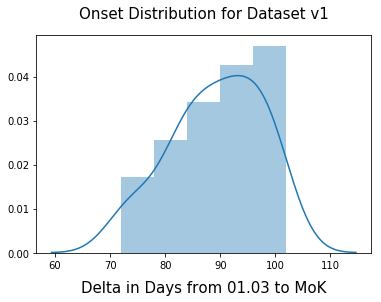
\includegraphics[width = 0.35\linewidth]{./99_appendix/img/onset_hist_v1}} &
    \subfloat{
      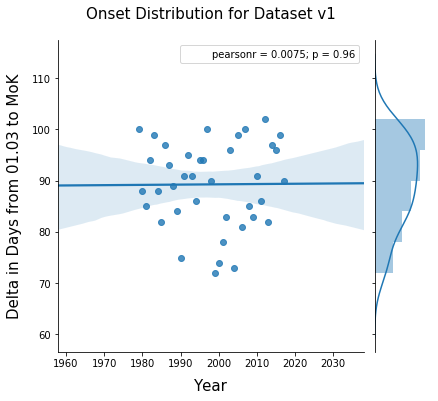
\includegraphics[width = 0.4\linewidth]{./99_appendix/img/onset_joint_v1}} \\
    \subfloat{
      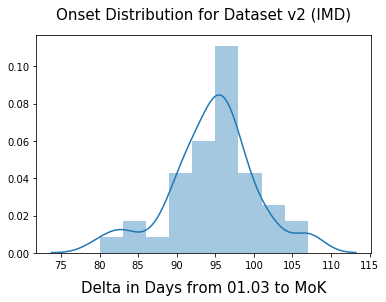
\includegraphics[width = 0.35\linewidth]{./99_appendix/img/onset_hist_v2_imd}} &
    \subfloat{
      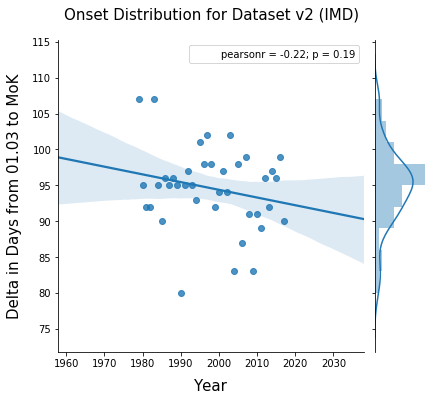
\includegraphics[width = 0.4\linewidth]{./99_appendix/img/onset_joint_v2_imd}} \\
    \subfloat{
      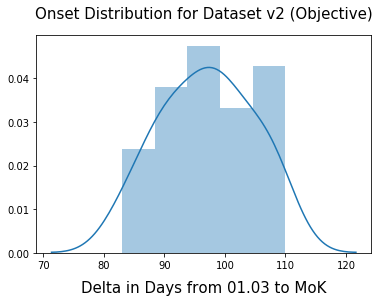
\includegraphics[width = 0.35\linewidth]{./99_appendix/img/onset_hist_v2_obj}} &
    \subfloat{
      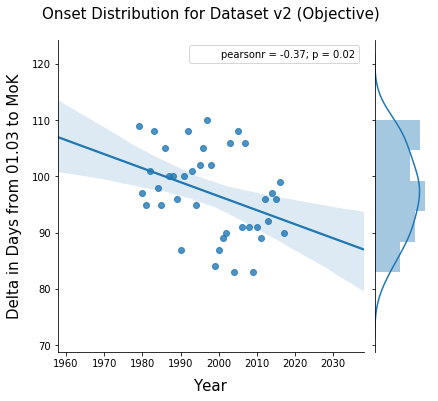
\includegraphics[width = 0.4\linewidth]{./99_appendix/img/onset_joint_v2_obj}} \\
  \end{tabular}
  \caption{Overview of Onset Distributions (1979-2017, v1: \citet{Ordonez.2016, IndiaMeteorologicalDepartment.2017b}, v2: \citet{Singh.2009, IndiaMeteorologicalDepartment.2017b}}
  \label{apx:onset_distributions}
\end{figure}

\begin{figure}[h]
  \centering
  \begin{tabular}{cc}
    \subfloat{
      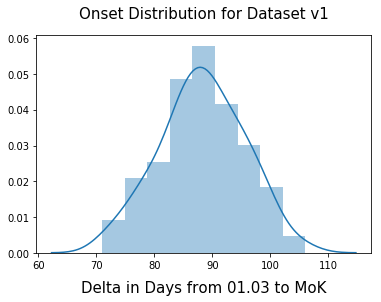
\includegraphics[width = 0.35\linewidth]{./99_appendix/img/onset_hist_v1_uncut}} &
    \subfloat{
      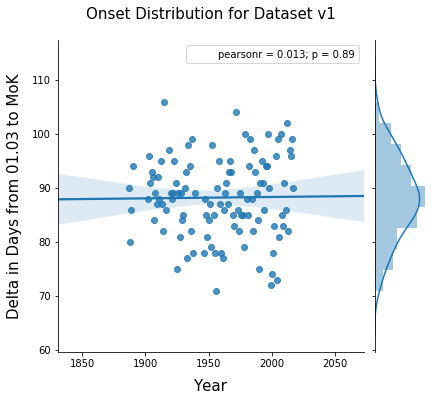
\includegraphics[width = 0.4\linewidth]{./99_appendix/img/onset_joint_v1_uncut}} \\
    \subfloat{
      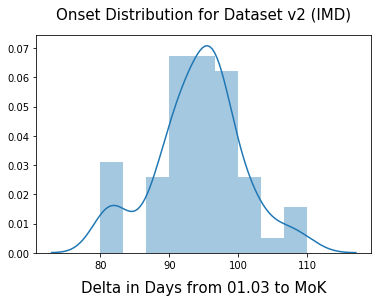
\includegraphics[width = 0.35\linewidth]{./99_appendix/img/onset_hist_v2_imd_uncut}} &
    \subfloat{
      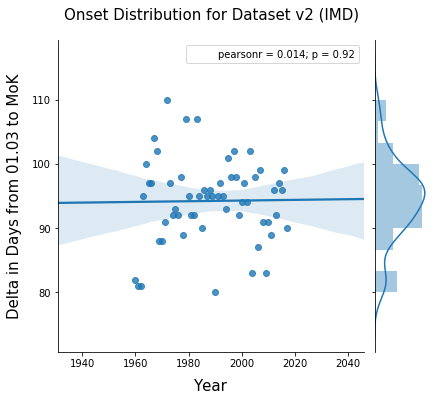
\includegraphics[width = 0.4\linewidth]{./99_appendix/img/onset_joint_v2_imd_uncut}} \\
    \subfloat{
      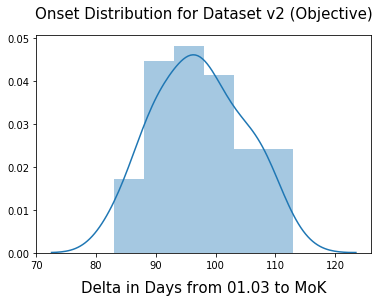
\includegraphics[width = 0.35\linewidth]{./99_appendix/img/onset_hist_v2_obj_uncut}} &
    \subfloat{
      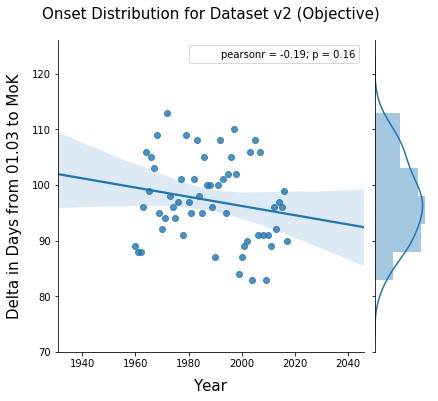
\includegraphics[width = 0.4\linewidth]{./99_appendix/img/onset_joint_v2_obj_uncut}} \\
  \end{tabular}
  \caption{Overview of Onset Distributions (v1: 1887-2017, \citet{Ordonez.2016, IndiaMeteorologicalDepartment.2017b}, v2: 1960-2017, \citet{Singh.2009, IndiaMeteorologicalDepartment.2017b})}
  \label{apx:onset_distributions_uncut}
\end{figure}

\clearpage
\section{TRMM \& ERA}
\label{apx:trmm_era}

\subsection{Getting the Datasets}
\label{apx:download}
\begin{itemize}
  \item TODO: Subsetting and Downloading (with Giovanni etc.)
\end{itemize}

\subsection{Usage with Python}
\begin{itemize}
  \item TODO: NetCDF4 vs. GRIB
  \item TODO: Python Libraries for handling NetCDF4
  \item TODO: Pseudocode for import
\end{itemize}

\clearpage
\subsection{Feature Analysis}

The visualizations in this section show the development of different ERA and TRMM features over the duration of an average monsoon. To calculate the visualizations, the data for each feature has been averaged over all years of available data (1998-2017 for TRMM, 1979-2017 for ERA).

\textbf{Example:} The temperature grids 10 days previous to the objective onset dates (Monsoon over Kerala, MoK; \ref{apx:era_t}) for all available years are extracted and then averaged to yield an averaged grid representation. The visualization is then simply calculated based on the averaged grid.

\begin{figure}[h]
  \centering
  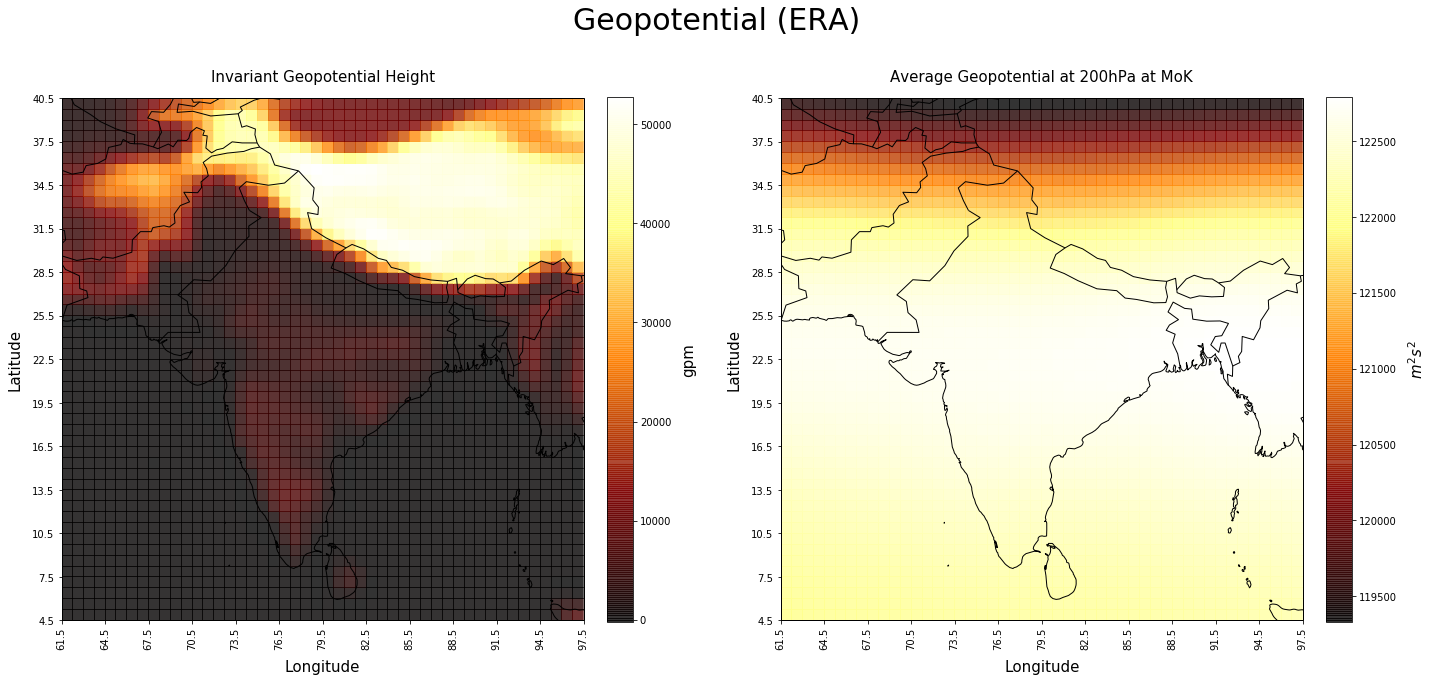
\includegraphics[width=\linewidth]{./99_appendix/img/geopotential}
  \caption{Geopotential Height and Geopotential at 200hPa (ERA-Interim, 1979-2017)}
  \label{apx:era_geopotential}
\end{figure}

\begin{figure}[h]
  \centering
  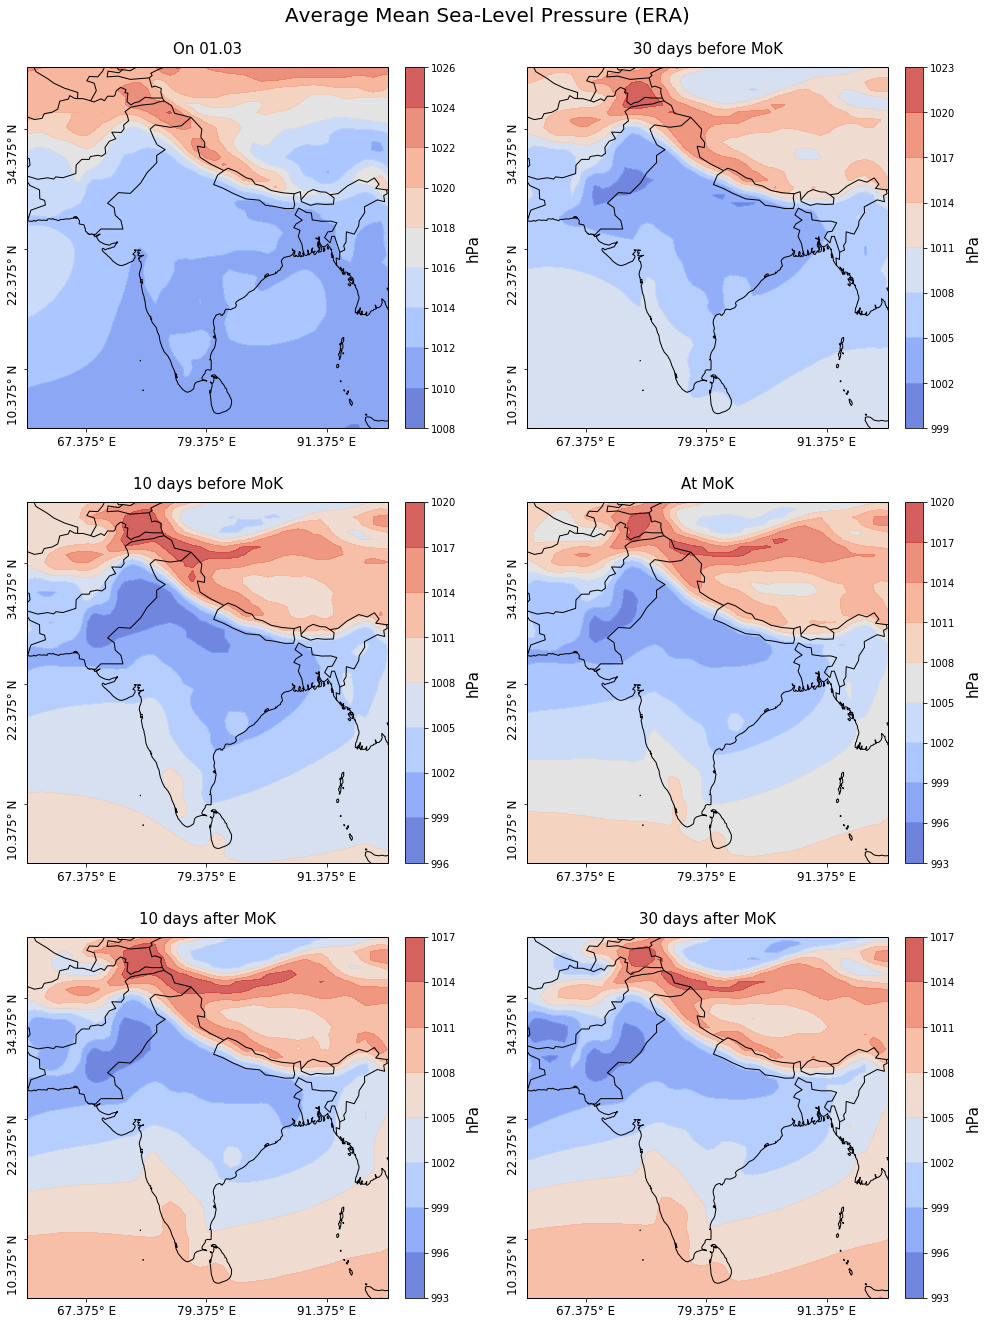
\includegraphics[width=\linewidth]{./99_appendix/img/msl_avg}
  \caption{Average Mean Sea-Level Pressure (ERA-Interim, 1979-2017)}
  \label{apx:era_msl}
\end{figure}

\begin{figure}[h]
  \centering
  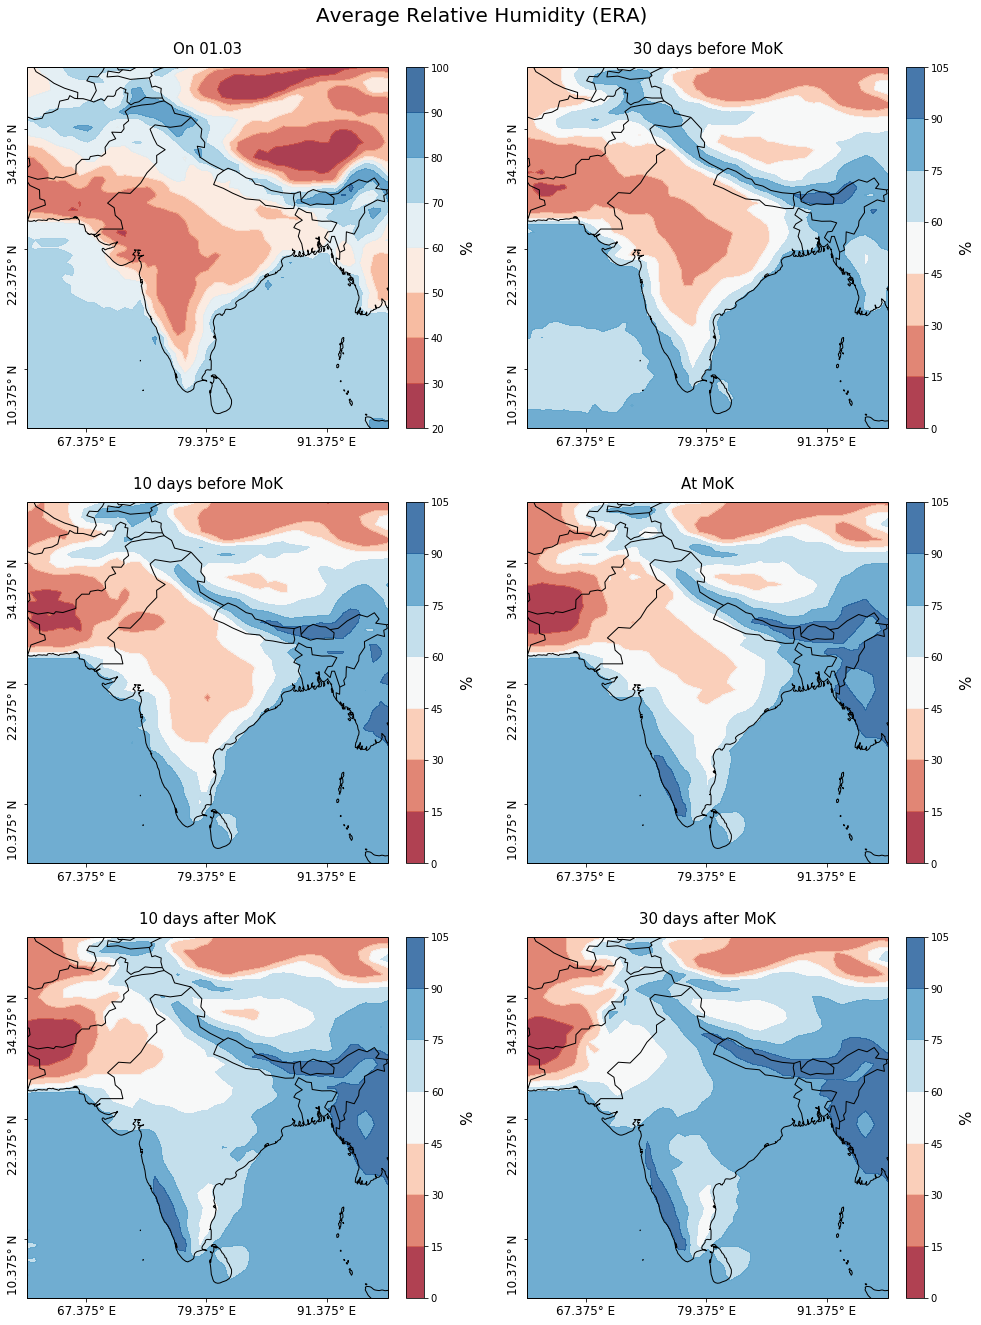
\includegraphics[width=\linewidth]{./99_appendix/img/r_avg}
  \caption{Average Relative Humidity at 1000hPa (ERA-Interim, 1979-2017)}
  \label{apx:era_r}
\end{figure}

\begin{figure}[h]
  \centering
  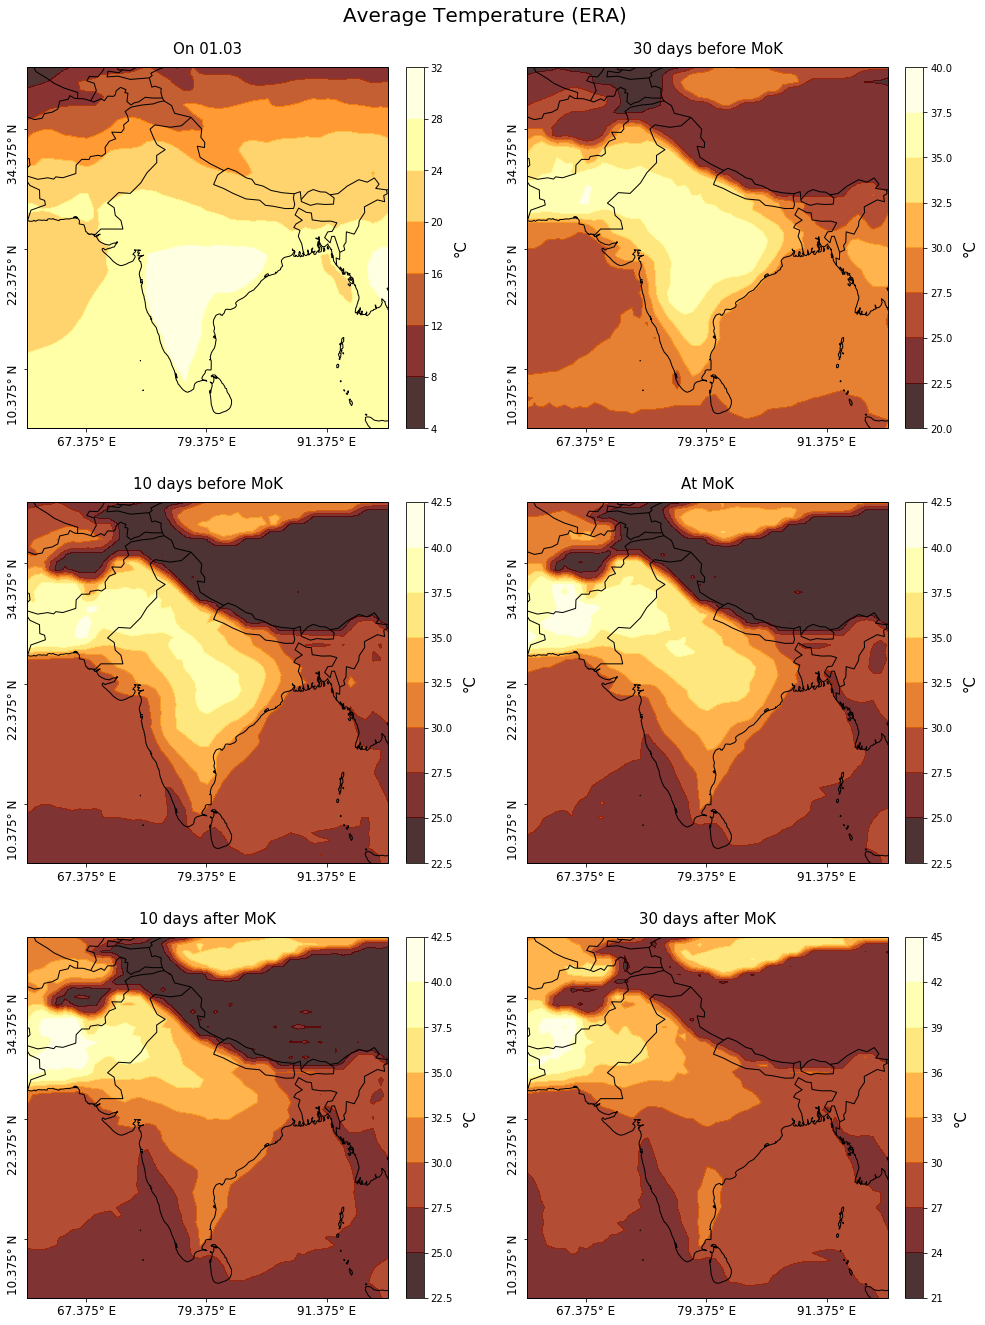
\includegraphics[width=\linewidth]{./99_appendix/img/t_avg}
  \caption{Average Temperature at 1000hPa (ERA-Interim, 1979-2017)}
  \label{apx:era_t}
\end{figure}

\begin{figure}[h]
  \centering
  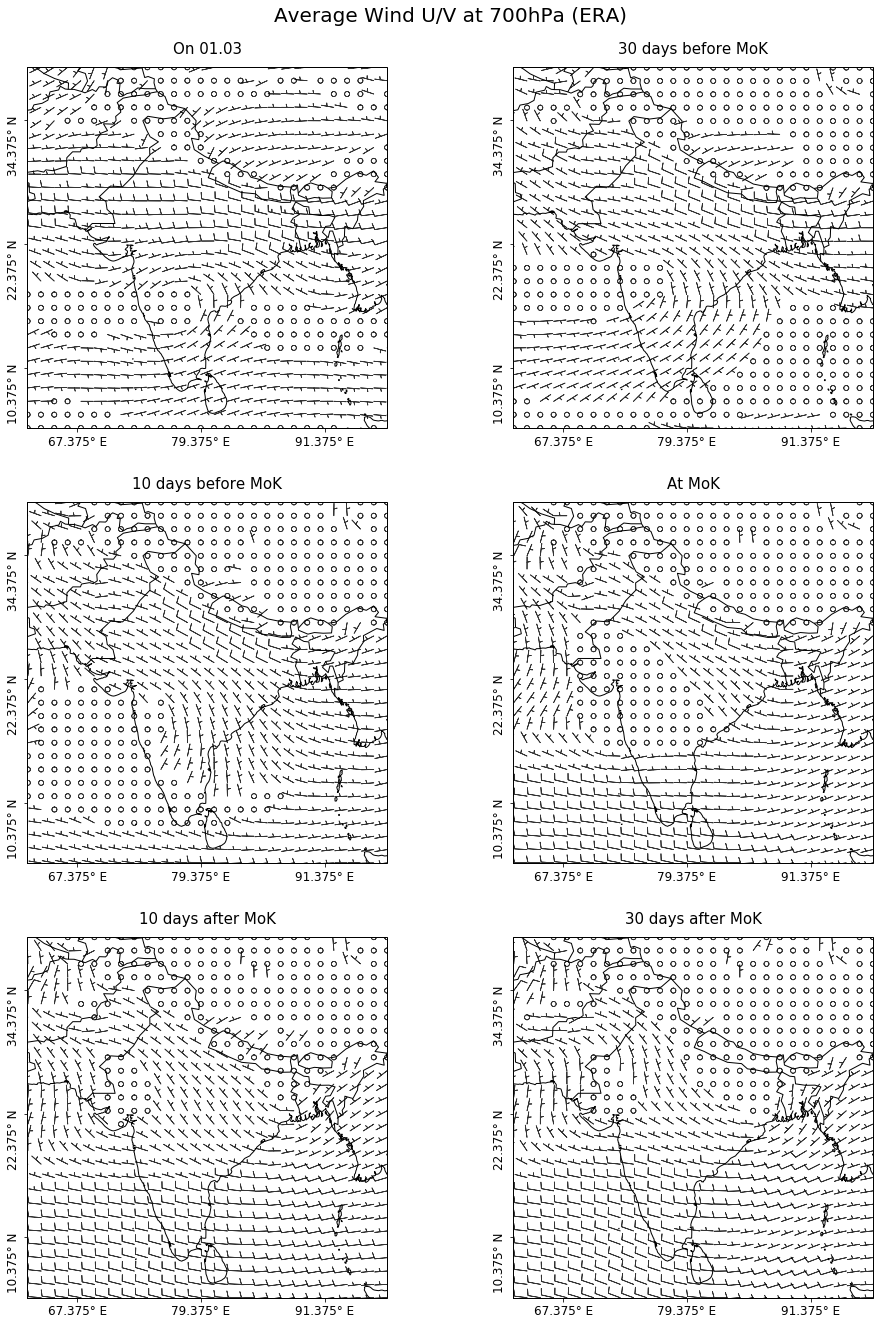
\includegraphics[width=\linewidth]{./99_appendix/img/wind_avg}
  \caption{Average Wind (U/V) at 700hPa (ERA-Interim, 1979-2017)}
  \label{apx:era_wind}
\end{figure}

\begin{figure}[h]
  \centering
  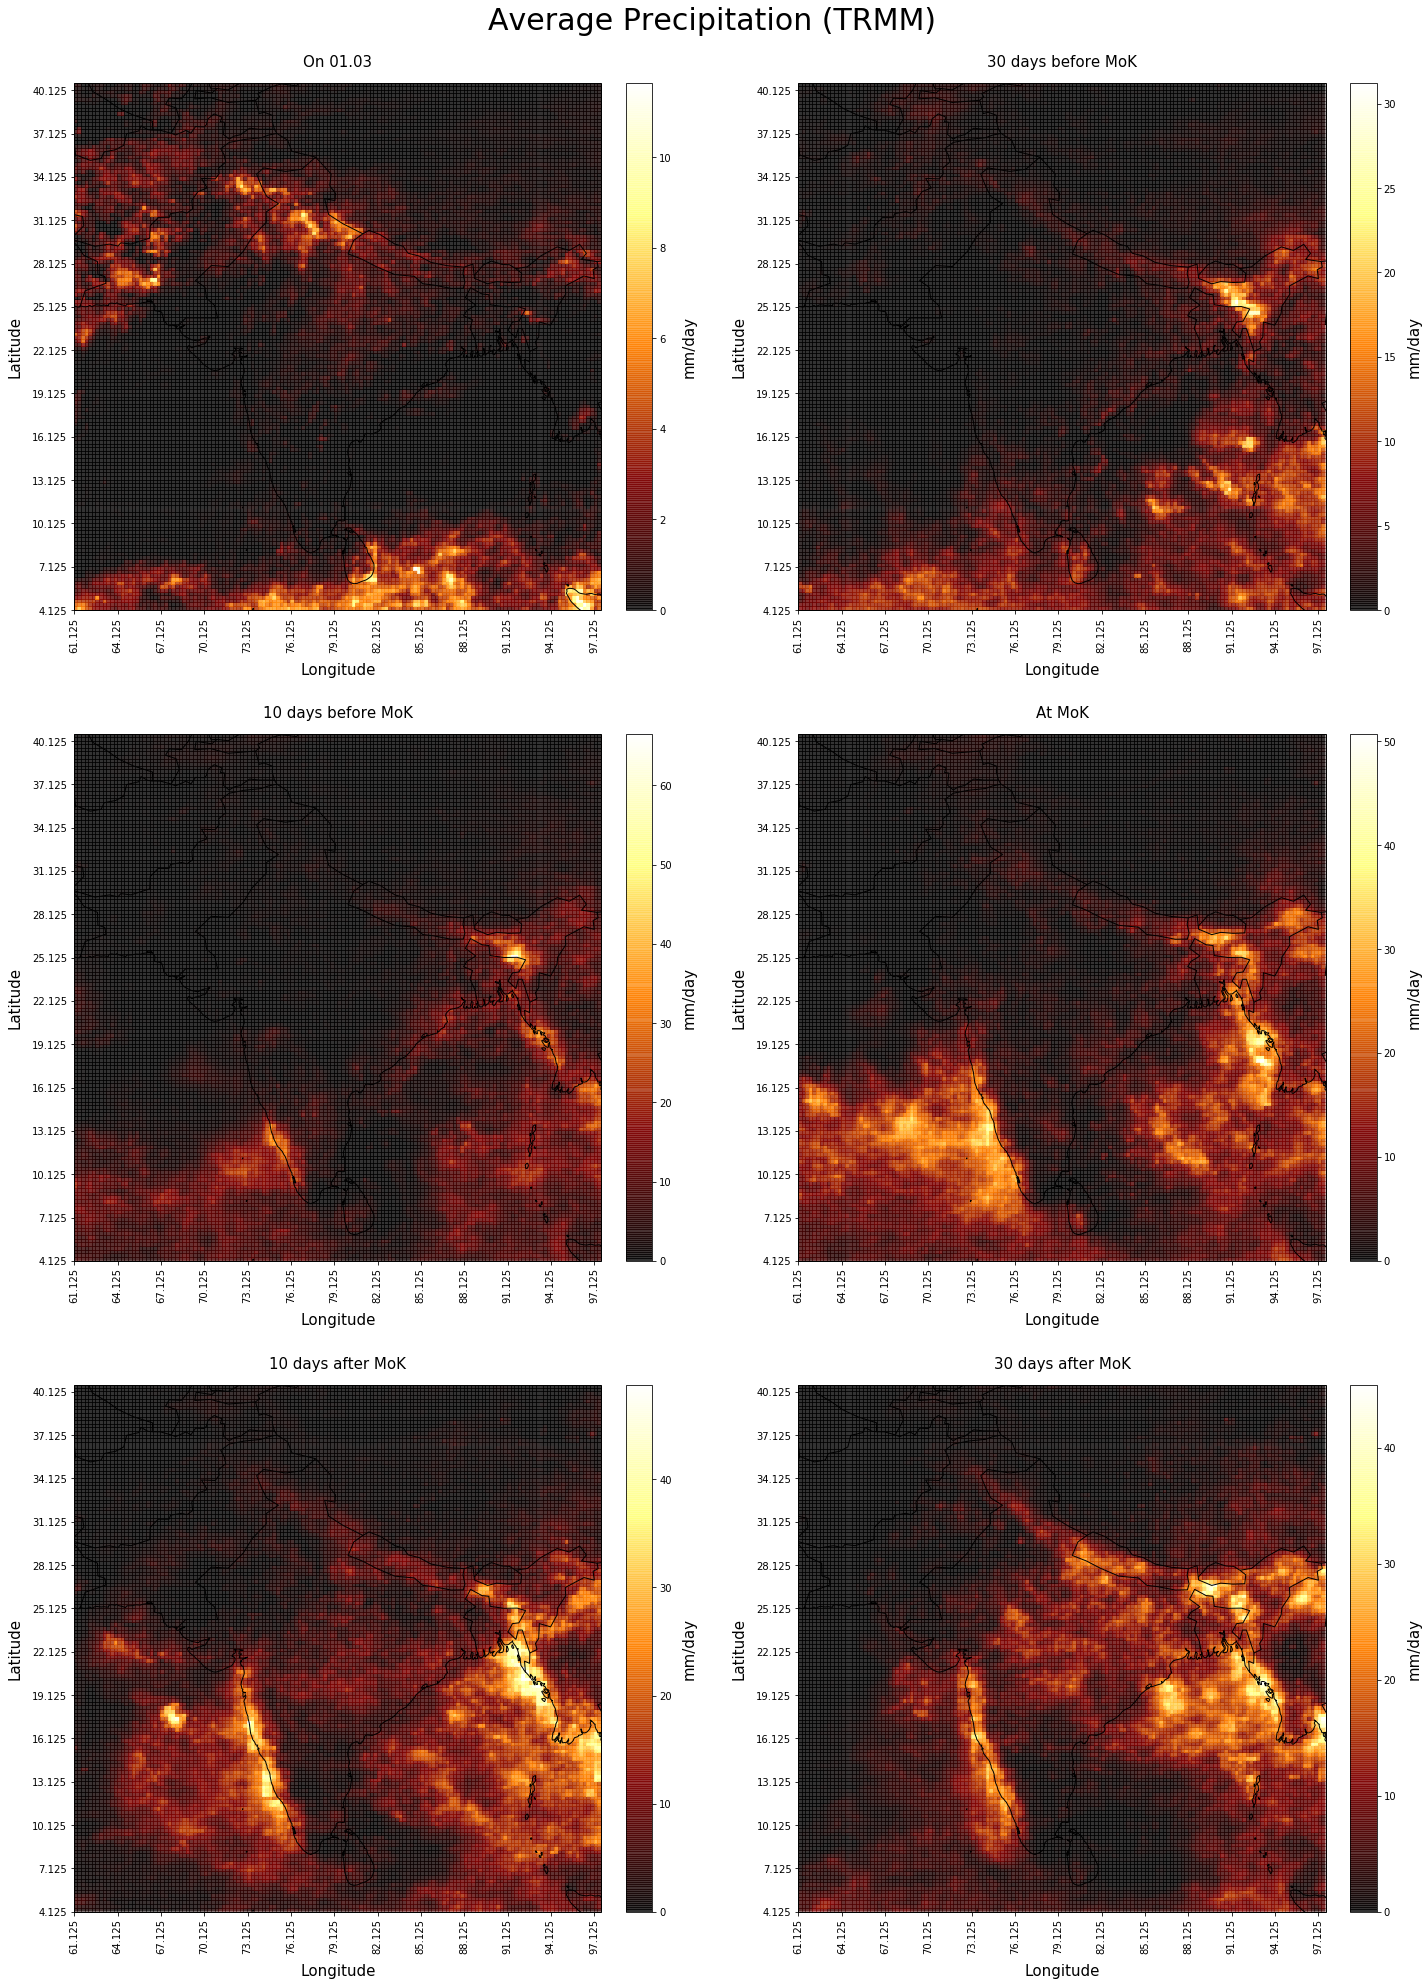
\includegraphics[width=\linewidth]{./99_appendix/img/prec_avg}
  \caption{Average Precipitation (TRMM, 1998-2017)}
  \label{apx:trmm_prec}
\end{figure}

\clearpage
\section{Event Synchronization}
\label{apx:event_sync}

[TODO: labels for rows (degree, betweenness, PageRank)]

\begin{figure}[h]
  \centering
  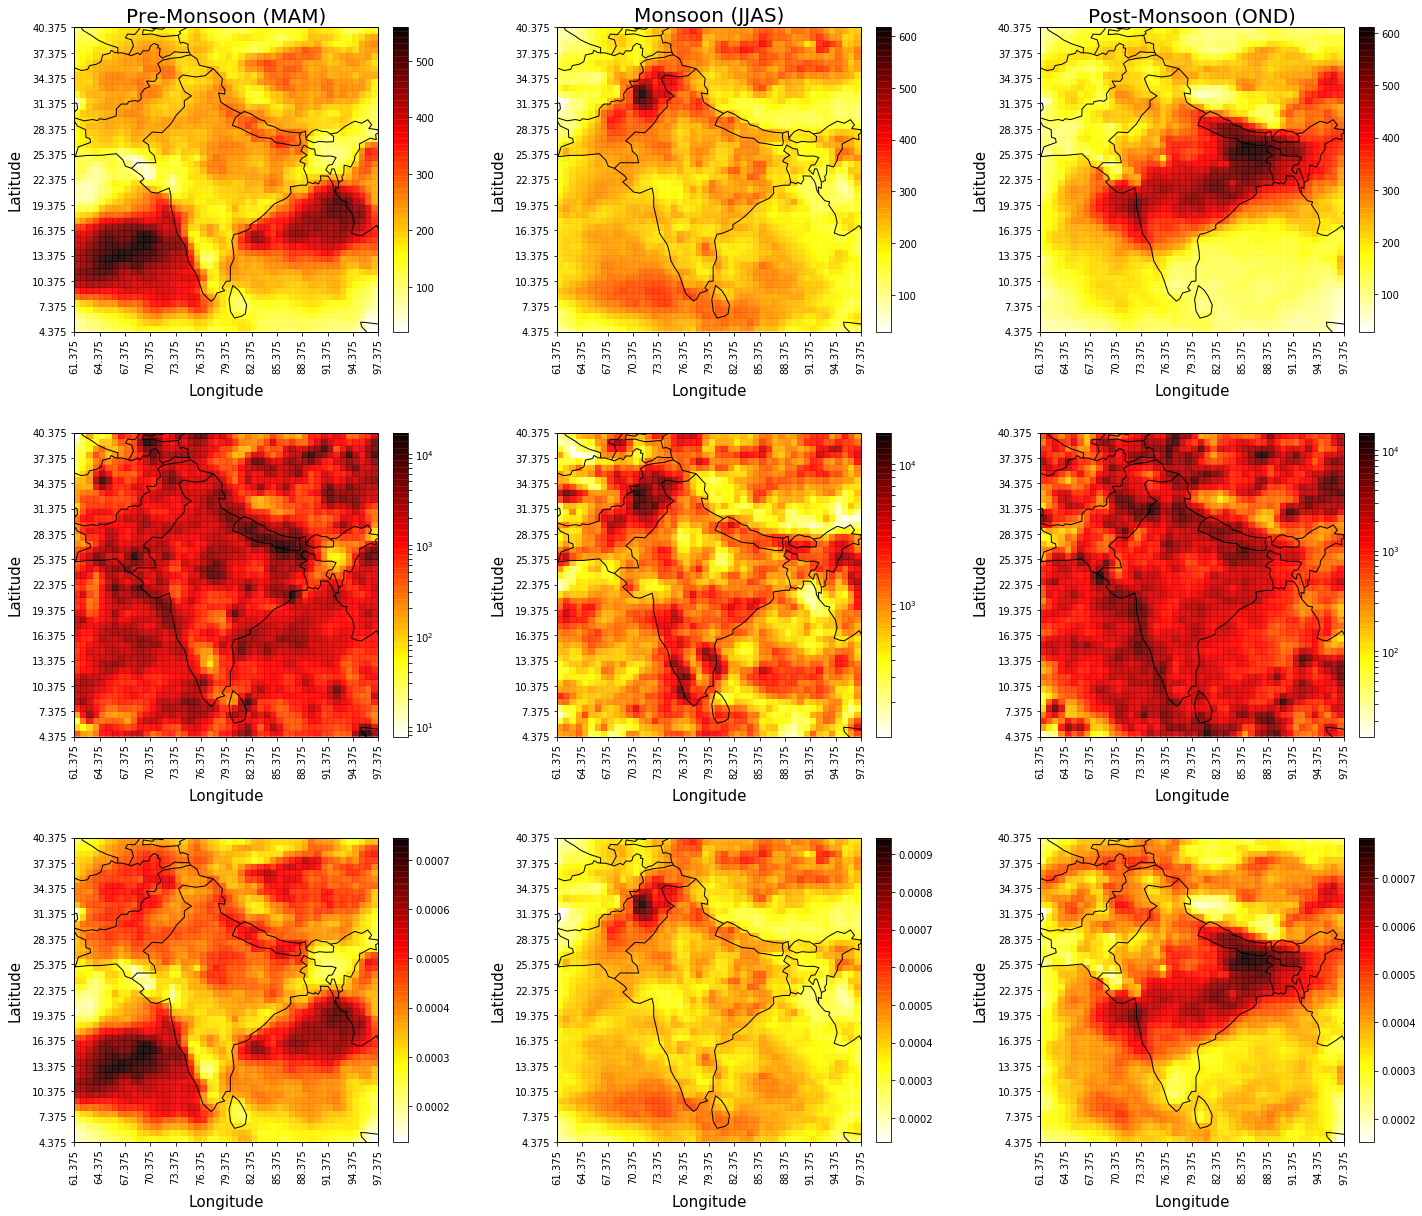
\includegraphics[width=\linewidth]{./99_appendix/img/event_sync_0-75_0-9.png}
  \caption{Event synchronization for unweighted climate networks}
  \label{apx:trmm_prec}
\end{figure}

\begin{figure}[h]
  \centering
  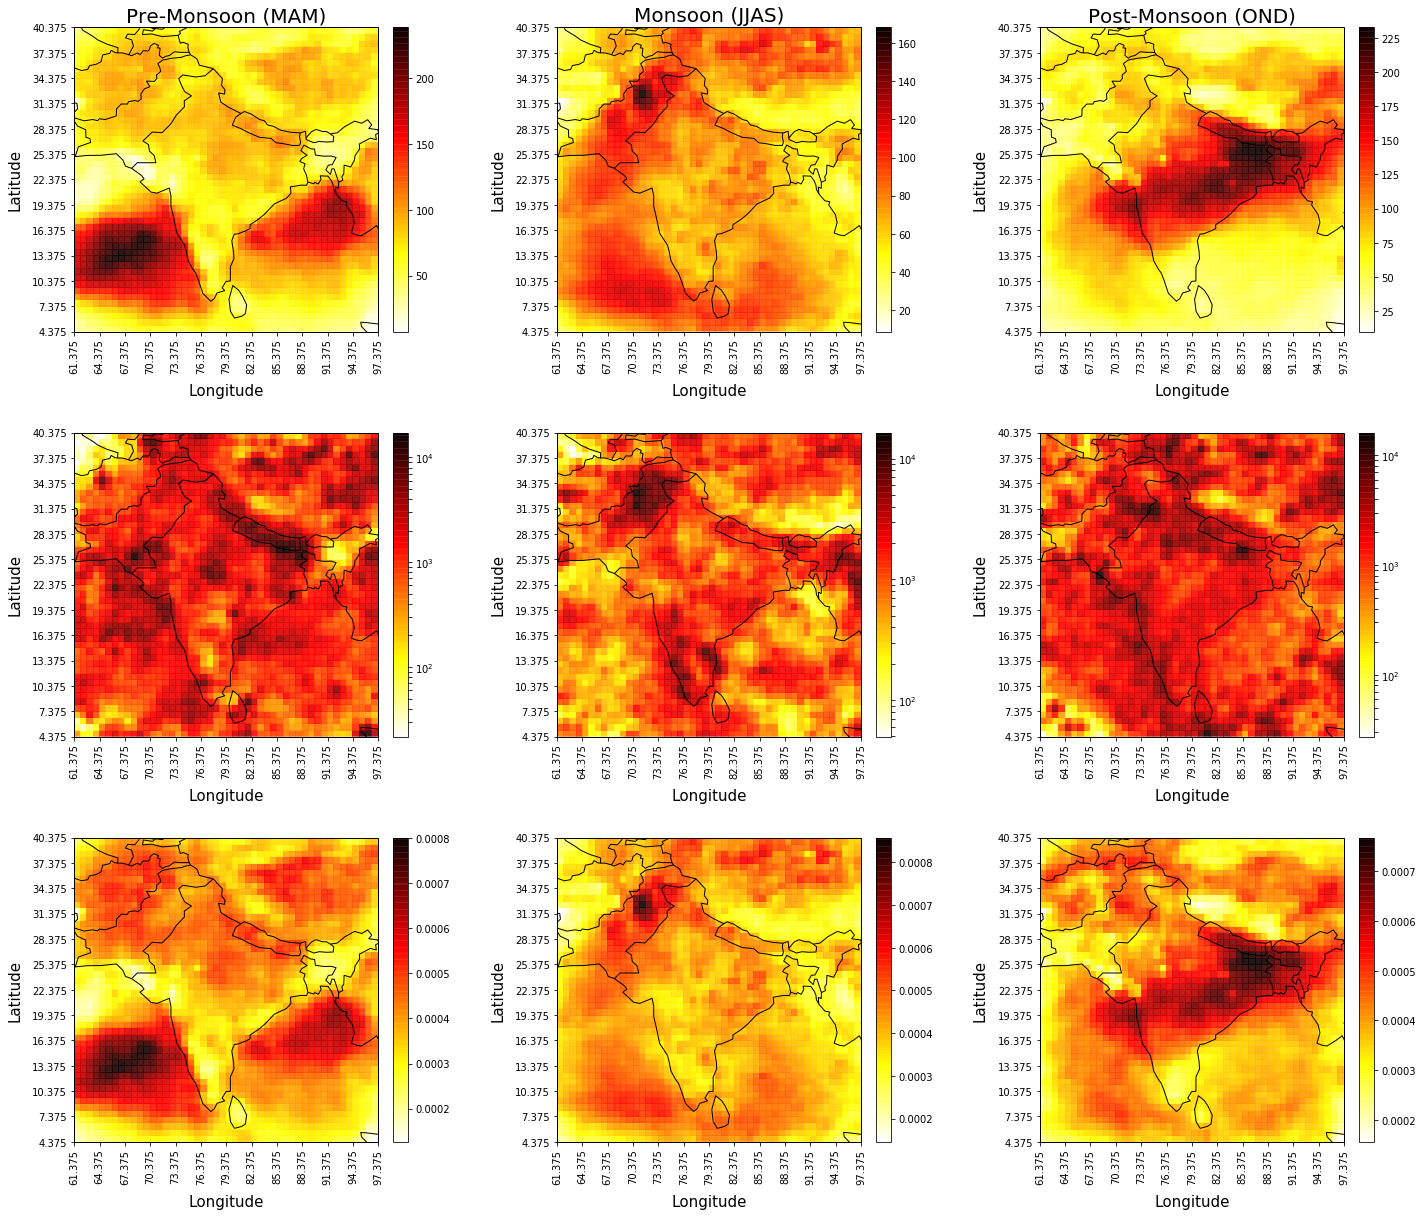
\includegraphics[width=\linewidth]{./99_appendix/img/event_sync_0-75_0-9_weighted.png}
  \caption{Event synchronization for weighted climate networks}
  \label{apx:trmm_prec}
\end{figure}


% *************** Back matter ***************
\backmatter

\normalfont
\clearpage
\listoffigures

\clearpage
\listoftables


\end{document}